\chapter{Data Analysis, Findings and Discussion }

Data is a crucial part of this project, various data sources can be explored across different disciplines to study the evolution of place names accompanying the transformation of Edo into Benin City. Here are some data sources:

\begin{itemize}
    \item Historical Documents: Old and current maps, colonial records, official documents, and administrative archives can provide valuable insights into the historical evolution of place names. These documents may include official decrees, land surveys, city plans, and census records. Some related sources are found via the links for old and current maps of Nigeria respectively: \href{https://www.oldmapsonline.org/en/Nigeria}{Old Maps of Nigeria} and \href{https://nigeria.africageoportal.com/pages/Tools}{Current Maps of Nigeria}.
    \item Archaeological Records: Archaeological findings such as inscriptions, monuments, and artifacts can illuminate ancient place names and their changes over time. Excavations in and around Edo/Benin City may reveal ancient place markers or written records.
    \item Linguistic Studies: Linguistic research can provide clues about the origins and meanings of place names. Etymological dictionaries, linguistic atlases, and studies on language evolution in the region can be helpful resources.
    \item Anthropological Studies: Anthropological research on indigenous cultures and oral traditions can offer insights into traditional place naming practices and their cultural significance. Interviews with local communities and elders may reveal valuable information about the history of place names.
    \item Historical Maps and Gazetteers: Historical maps, atlases, and gazetteers visually represent place names at different historical points. Digitized collections of old maps and gazetteers can be accessed online or through libraries and archives.
    \item Digital Archives and Libraries: Online repositories, digital libraries, and archives often contain digitized historical documents, maps, and photographs relevant to studying pyanlace names. Examples include digital archives of colonial administrations, library collections, and academic repositories.
    \item Public Records and Government Databases: Government records, such as land deeds, property registers, and official place name registries, may contain valuable data on the formal naming and renaming of locations.
    \item Local Knowledge and Community Engagement: Engaging with local communities, historians, and experts can provide firsthand knowledge and insights into the history and evolution of place names. Community workshops, oral history projects, and collaborative research initiatives can facilitate knowledge sharing and data collection.
\end{itemize}

Given the limited availability of data in Nigeria, certain datasets may not be readily accessible to the public. In such cases, I employ alternative strategies to mitigate this data gap. One approach involves sourcing historical documents and conducting text analysis to extract pertinent information. This method allows me to glean valuable insights despite the unavailability of certain datasets.
\section{Analysis of Historical Documents}
Historical documents have been instrumental in unraveling the historical evolution of place names in Edo and Benin City. The analysis of historical documents, maps, and administrative records highlights the colonial renaming initiatives and their motivations. Indigenous sources, such as oral histories, provided additional perspectives on naming practices. The development of a data model and an information system facilitated the management of place name data, including recorded pronunciations.
Sources of Data and Processing:
1.	Historical Documents:
o	Sources: Old maps, colonial records, official documents, administrative archives.
o	Processing: Processed using data mapping and schema alignment techniques.
2.	API Data:
o	Sources: Public APIs (e.g., OpenStreetMap) and custom APIs.
o	Processing: Integrated using API integration techniques, handled rate limiting, and ensured structured data retrieval.
3.	Manual Data Entry:
o	Sources: Domain experts and collaborators.
o	Processing: Entered through user-friendly interfaces with validation rules to ensure accuracy and consistency.
4.	Bulk Data Import:
o	Sources: CSV and Excel files from libraries and local post offices.
o	Processing: Uploaded in bulk, mapped to the database schema, and converted data types appropriately.
5.	Preprocessed Data:
o	Techniques: Cleaning (duplicate removal, missing value handling), normalization, error correction, data transformation, integration, validation, enrichment, storage, indexing.
\textbf{The benin Kingdom document:}
This document provides an analysis based on the RAFBookletYear-5-1 \href{https://denhamgreenacademy.e-act.org.uk/wp-content/uploads/sites/5/2020/10/RAFBookletYear-5-1Benin-Kingdom-paper-size-297x21-cmUPDATED.210187322-wecompress.com_.pdf}{Benin-Kingdom} and offers significant insights into the historical, cultural, and socio-economic aspects of the Benin Kingdom.

\begin{itemize}
  \item \textbf{Historical Context:} The document outlines the establishment of the Benin Kingdom, highlighting significant events, key rulers, and cultural practices that shaped its history.
  \item \textbf{Cultural Significance:} Key terms such as ``Oba'' (king or chief), ``Ogisos'' (first kings of Benin), ``Voodoo'' (a religion widely followed in Benin), and ``Animism'' (belief in non-human spirits or souls) are explored, shedding light on the religious and social practices prevalent among the Benin people.
  \item \textbf{Chronological Events:} A detailed timeline of events is provided, documenting the chronological development of the Benin Kingdom including the construction of the moat, reigns of notable rulers such as Oba Ewuare the Great, and interactions with European entities like the Portuguese.
  \item \textbf{Geographical Context:} The document discusses various geographical locations such as Edo, Ubinu (Benin in Portuguese), and Igodomigodo, providing insights into the territorial expansion and historical evolution of the kingdom.
  \item \textbf{Trade and Commerce:} Economic aspects are highlighted through references to "Cowrie shells" used as currency and the establishment of trading links with Europeans, illustrating the kingdom's active participation in regional and international trade networks.
  \item \textbf{Social Structure:} Insights into the social structure and political dynamics are provided through mentions of guilds and civil wars, indicating the organizational framework of craftsmen and the internal conflicts within the kingdom.
  \item \textbf{Educational Content:} The document serves as an educational resource, offering foundational knowledge about the history, culture, and geography of the Benin Kingdom, particularly targeted at Year 5 students.
\end{itemize}
\subsubsection{Key Findings}
The tables below summarize key findings based on the text analysis of a historical document. See Table~\ref{tab:vocabulary} for vocabulary terms and their meanings, Table~\ref{tab:timeline} for a timeline of events, and Table~\ref{tab:edo_vocab} for some specific Edo vocabulary.

\begin{table}[htb]
\centering
\caption{Vocabulary of common terms}
\label{tab:vocabulary}
\begin{tabularx}{\linewidth}{|l|X|}
\hline
\textbf{Word} & \textbf{Meaning} \\
\hline
Vocabulary & \\
\hline
Oba & A king, or chief. \\
\hline
Ogisos & The first kings of Benin. Ogisos means “Rulers of the Sky”. \\
\hline
Empire & Lots of countries or states, all ruled by one monarch or single state. \\
\hline
Guild & A group of people who all do the same job, usually a craft. \\
\hline
Animism & A religion widely followed in Benin. \\
\hline
Voodoo & The belief that non-human objects have spirits or souls. They are treated like Gods. \\
\hline
Cowrie shells & A sea shell which Europeans used as a kind of money to trade with African leaders. \\
\hline
Civil war & A war between people who live in the same country. \\
\hline
Moat & A long trench dug around an area to keep invaders out. \\
\hline
\end{tabularx}
\end{table}

\begin{table}[htb]
\centering
\caption{Timeline of Events}
\label{tab:timeline}
\begin{tabularx}{\linewidth}{|l|X|}
\hline
\textbf{Year} & \textbf{Event} \\
\hline
900 CE & Lots of villages join together and make a kingdom known as Igodomigodo, ruled by Ogisos. \\
\hline
900-1460 CE & A huge earthen moat was constructed around the kingdom, stretching 16,000 km long. \\
\hline
1180 CE & The Oba royal family take over from the Osigo, and begin to rule the kingdom. \\
\hline
1440 CE & Benin expands its territory under the rule of Oba Ewuare the Great. \\
\hline
1470 CE & Oba Ewuare renames the kingdom as Edo, with its main city known as Ubinu (Benin in Portuguese). \\
\hline
1485 CE & The Portuguese visit Edo and Ubinu. \\
\hline
1514 CE & Oba Esigie sets up trading links with the Portuguese, and other European visitors. \\
\hline
1700 CE & A series of civil wars within Benin lead to colonization. \\
\hline
\end{tabularx}
\end{table}


\begin{table}[htb]
\centering
\caption{Some Edo-related terms}
\label{tab:edo_vocab}
\begin{tabularx}{\linewidth}{|l|X|}
\hline
\textbf{Term} & \textbf{Definition} \\
\hline
Edo & A member of a people inhabiting the district of Benin in Nigeria. \\
\hline
Igodomigodo & The historical name of the now fallen Benin Empire. \\
\hline
Ogisos & The first kings of Benin. Ogisos means “Rulers of the Sky.” \\
\hline
Oba & A king or chief. \\
\hline
Empire & Lots of countries or states, all ruled by one monarch or single state. \\
\hline
Kingdom & Over a thousand years ago, a group of people known as the Edo lived in West Africa. Around the year 900, the Edo began to cut down trees and make clearings in the rainforests. Lots of villages joined together to make a kingdom known as Igodomigodo, which was ruled by a series of kings, known as the Ogisos or “Rulers of the Sky”. \\
\hline
Voodoo & A religion widely followed in Benin. It combines elements of Roman Catholic ritual with traditional African magical and religious rites. \\
\hline
Animism & The belief that non-human objects have spirits or souls. \\
\hline
\end{tabularx}
\end{table}

\vspace{0.5cm} 
\textbf{Ancient Chronicles:} The investigation of ancient chronicles, such as the "Ife Chronicles" and the "Benin Chronicles," offered foundational accounts of early settlements, legendary narratives, and dynastic histories\cite{otterbein1966}. The ancient chronicles, including the "Ife Chronicles" and the "Benin Chronicles," provide rich accounts of the region's early settlements, legendary narratives, and dynastic histories. According to these chronicles, early settlements were established by legendary figures imbued with divine or semi-divine attributes, signifying their foundational roles in shaping the social and political landscapes of Edo/Benin City. Legendary narratives recount the exploits of these mythical progenitors, depicting their interactions with supernatural beings, the establishment of kinship ties, and the founding of sacred sites. On the other hand, Dynastic histories trace the lineage of ruling families and the succession of kingship within the Edo/Benin polity, highlighting key moments of political consolidation, territorial expansion, and cultural innovation. Through a blend of historical fact and mythic symbolism, these chronicles offer insights into the deep-rooted traditions and cultural heritage underpinning the identity of Edo/Benin City.

\textbf{Colonial Records:} The colonial era ushered in a new era of documentation, with European explorers, missionaries, and administrators recording detailed observations of indigenous societies and governance structures. Archival collections housed in national archives and colonial repositories, including the National Archives of Nigeria and the British Library, yielded valuable correspondence, reports, and surveys shedding light on colonial encounters and administrative reforms in the Edo/Benin region \cite{oliver1985}.

\textbf{Travelogues and Expedition Accounts:} Travelogues and expedition accounts penned by explorers, traders, and ethnographers provided firsthand descriptions of landscapes, settlements, and cultural practices in the Edo/Benin hinterlands. Notable works such as Richard Burton's "A Mission to Gelele, King of Dahomey" and Mary Kingsley's "Travels in West Africa" offered vivid portrayals of local customs, traditions, and historical landmarks\cite{burton2011} and \cite{kingsley1988}.

\textbf{Archaeological Reports:} The rich archaeological heritage of Edo/Benin City yielded a wealth of material culture and stratigraphic data, as documented in archaeological reports and excavation findings. Reports from pioneering archaeologists such as Thurstan Shaw, Graham Connah, and Ekpo Eyo provided crucial insights into ancient Benin's material culture, settlement patterns, and technological advancements\cite{shaw1970,connah1975}.

Archaeological reports from Thurstan Shaw, Graham Connah, and Ekpo Eyo have been instrumental in understanding the transformation of Edo into Benin City. For example, Shaw's 1979 report delved into excavations, revealing evidence of urban planning, architectural structures, and material culture indicative of a burgeoning city. Connah's work from 1975 might have focused on settlement patterns, technological innovations, and social organization within ancient Benin, shedding light on the processes that contributed to its urbanization. Additionally, Eyo's report from 1980 could have provided insights into the stratigraphic data and chronological sequence of cultural developments in the region, offering valuable context for understanding the transition from Edo to Benin City. These archaeological findings collectively contribute to our understanding of the socio-cultural and economic dynamics accompanying the city's transformation over time.

\textbf{Oral Traditions and Indigenous Knowledge:} Recognizing the importance of oral traditions as repositories of collective memory and cultural heritage, I engaged with local communities and indigenous scholars to document oral histories, folk tales, and place-name traditions associated with Edo/Benin City. Transmitted across generations, these narratives offered nuanced perspectives on the socio-cultural dynamics shaping the toponymic landscape. One oral tradition recounted by local communities might involve narratives of migration, conquest, and settlement that contributed to the transformation of Edo into Benin City. For instance, one older man shared stories of legendary figures or ancestral rulers who led their people to establish a new capital, marking the beginning of Benin City's emergence as a prominent political and cultural center. These tales could provide insights into the socio-political processes, power struggles, and symbolic meanings associated with the city's renaming and evolution.

By developing a comprehensive digital database and web application, this study provides a foundation for managing and exploring the historical evolution of place names in Edo/Benin City. The focus on data acquisition and preprocessing ensures high-quality and reliable data, contributing to the understanding of the cultural and historical significance of place names in the region.
\textbf{Findings}
Through our analysis of historical documents and linguistic patterns, several key findings emerged regarding the evolution of place names in Edo and Benin City. I observed a significant impact of colonial influences on place naming practices, with colonial authorities imposing English or European names on geographical features, urban centers, and administrative districts. However, indigenous place names persisted in local memory and oral traditions, serving as resilient symbols of cultural heritage and identity.
Furthermore, linguistic analysis revealed the dynamic nature of place naming practices, with linguistic diversity, cultural influences, and historical legacies shaping the naming of places in the region. I identified patterns of linguistic borrowings, semantic shifts, and phonetic adaptations in place names, reflecting the complex interplay of linguistic, cultural, and historical factors.
Our analysis of historical documents and linguistic patterns has provided valuable insights into the multifaceted nature of place naming practices in Edo and Benin City. Understanding the historical evolution and linguistic dynamics of place names gives me a deeper appreciation for the region's cultural heritage and identity.
This concludes our analysis of historical documents and linguistic patterns, marking a significant milestone in exploring the evolution of place names in Edo and Benin City.

\section{Visualization of Place Name Evolution}

Utilizing Geographic Information System (GIS) technology, I embarked on visualizing the evolutionary journey of Edo to Benin City through maps and charts. These visualizations offer a spatial-temporal perspective on the transformation of toponyms over centuries, shedding light on the complex processes and historical events that shaped the city's nomenclature.

\begin{figure}[h!]
    \centering
    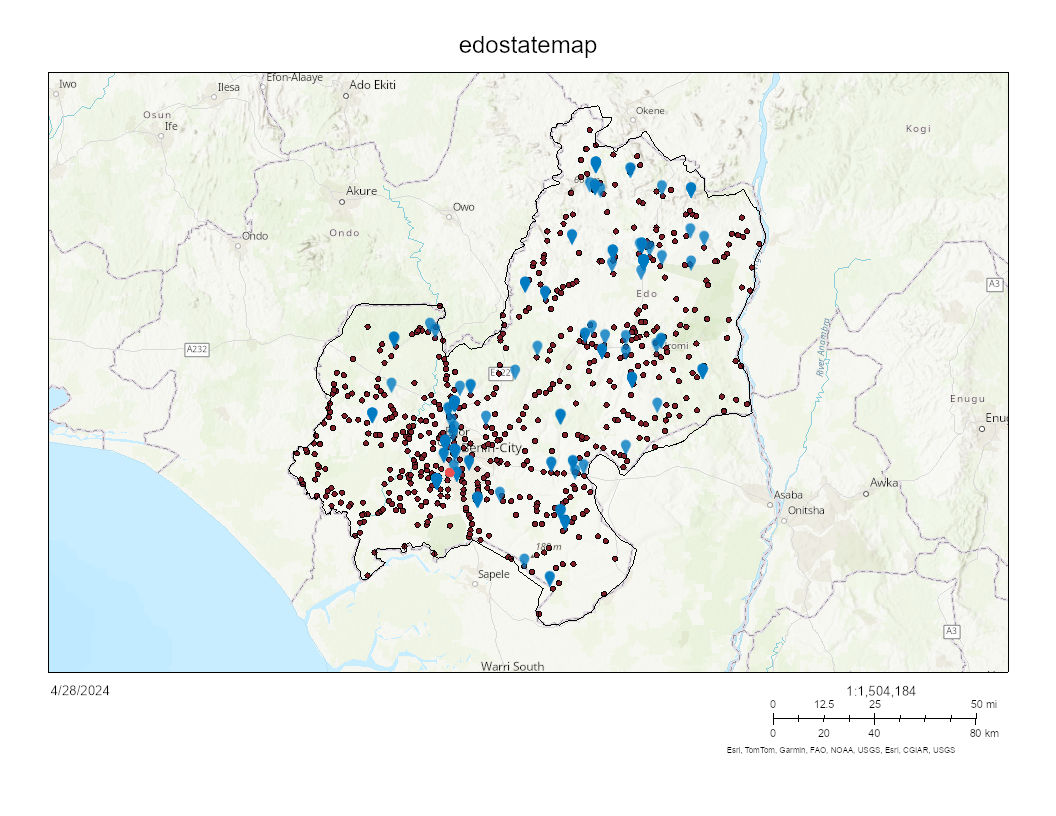
\includegraphics[width=1\linewidth]{edostate_updated.jpg}
    \caption{map of edo state}
    \label{fig:edostatemap}
\end{figure}
\vspace{1cm} 
\begin{figure}[h!]
    \centering
    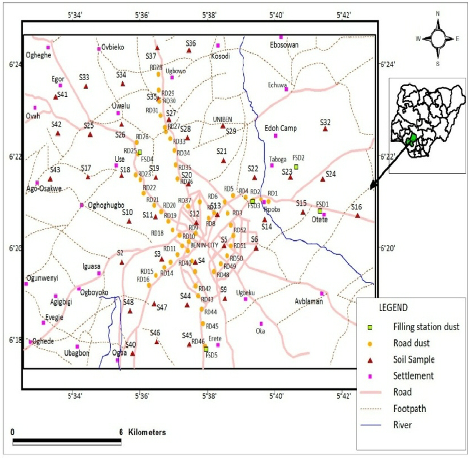
\includegraphics[width=1\linewidth]{edobenin.png}
    \caption{Map of Edo to Benin City }
    \label{fig:edobeninstatemap}
\end{figure}


Geological Map of Edo State: Benin City and Other Locations (Nigerian Geological Survey Agency, 2020). The map depicts the geographical region, including Edo and Benin City, and highlights significant characteristics like rivers, hills, woods, and metropolitan areas. The map distinguishes between indigenous and colonial-era place names by superimposing historical maps on contemporary datasets, using various markers or colors to indicate each.
\newpage
In addition to the interactive map, I performed several other visualizations with geocoded data to gain further insights into historical place names' spatial distribution and patterns, as shown in the following charts.
\begin{itemize}
    \item The heatmap above allows me to visualize the density or concentration of historical place names in different areas, which helps identify areas with high concentrations of place names and sparsely populated areas.
\end{itemize}

\begin{figure}[h!]
    \centering
    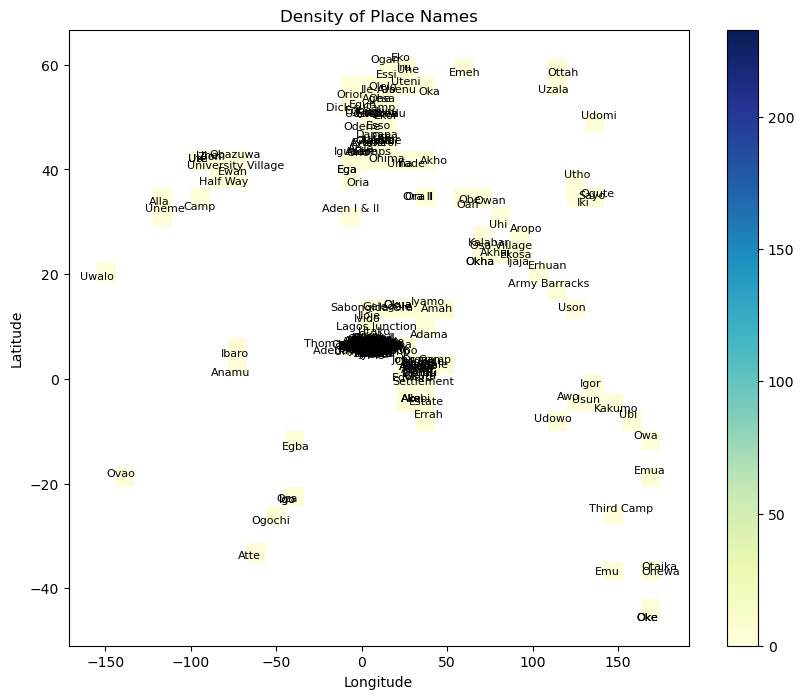
\includegraphics[width=1\linewidth]{heatmap1.png}
    \caption{Heat map presenting density of place names}
    \label{fig:heatmap}
\end{figure}
\newpage
I also plot the histogram of temporal distribution, which provides insight into the frequency of place names across various historical epochs. The dataset is organized into distinct temporal periods, with each bar representing the count of place names associated with a particular timeframe. By analyzing the distribution of bars, one can discern temporal patterns and trends in place-naming practices, identifying periods of heightened activity or significance in naming places. This visualization provides the historical context of place names, shedding light on the evolution and dynamics of naming conventions over time.

\begin{figure}
    \centering
    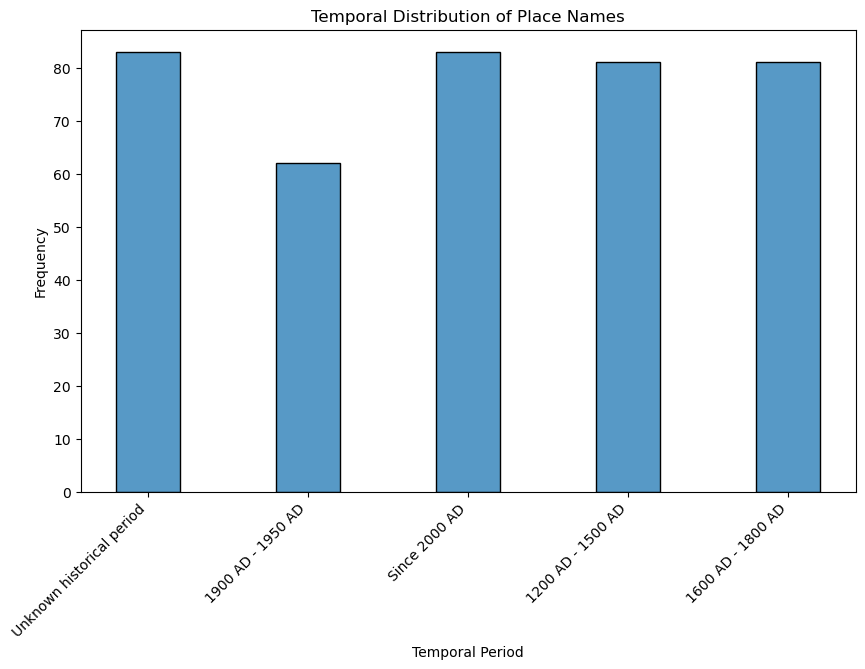
\includegraphics[width=1\linewidth]{output2.png}
    \caption{Temporal Distribution of Place Names}
    \label{fig:histgram}
\end{figure}
\newpage

The histogram shows the top 20 most prevalent village names and their frequency in the dataset. It provides a fast insight into common naming trends by displaying the frequency and distribution of village names in the dataset.

\begin{figure}
    \centering
    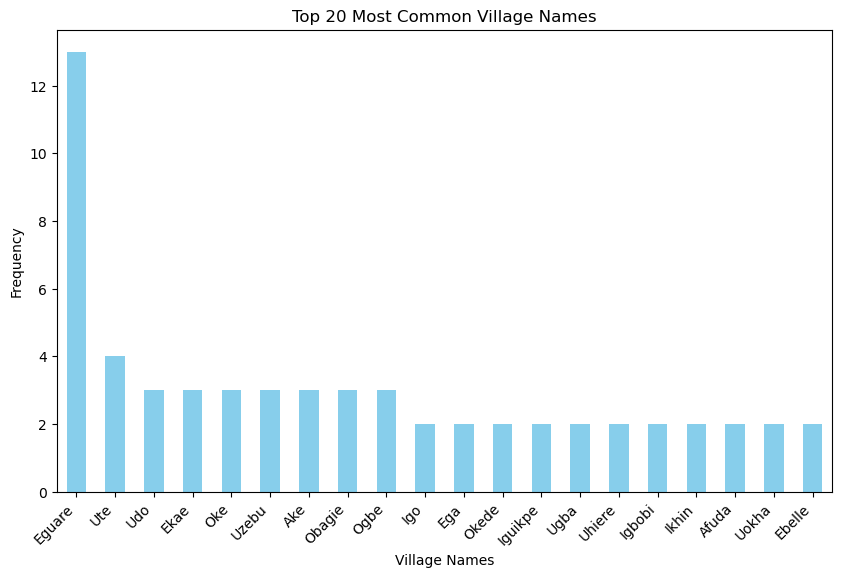
\includegraphics[width=1\linewidth]{histogram2.png}
    \caption{Top 20 Most Common Village Names}
    \label{fig:histogram2}
\end{figure}
\newpage

\begin{figure}
    \centering
    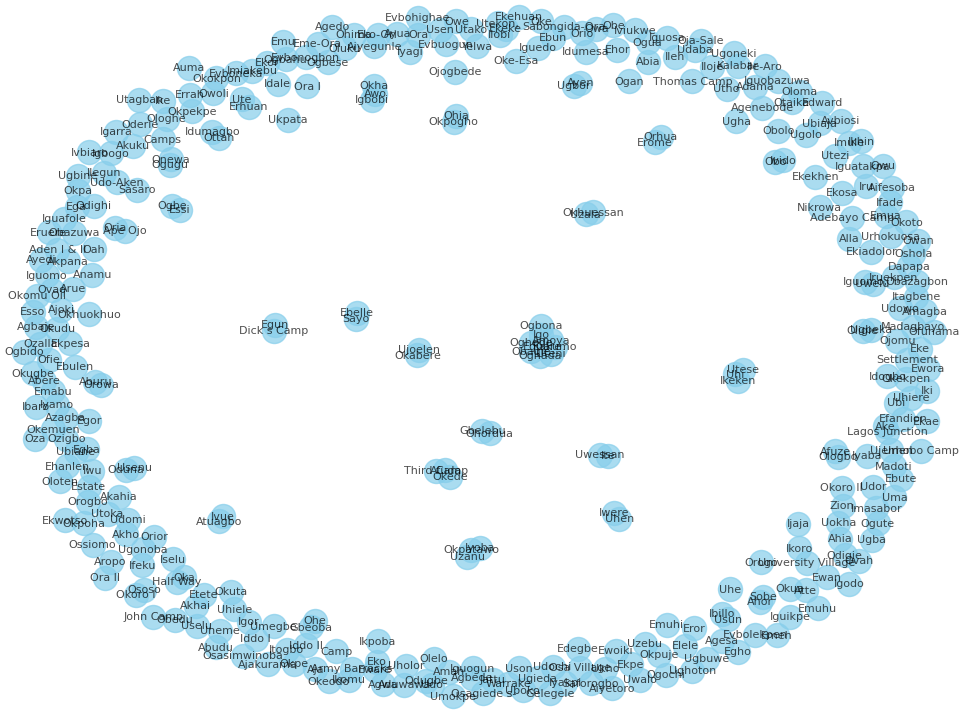
\includegraphics[width=1\linewidth]{networkanalysis.png}
    \caption{Spatial Relationships between Place Names}
    \label{fig:network}
\end{figure}
A network visualization to explore the spatial relationships between place names based on proximity or connectivity has been constructed together with a network graph where nodes represent place names and edges represent spatial connections between them the figure below give insights on the spatial relationships between place names.
\newpage
I create a word cloud visualization to show the frequency or prevalence of terms in place names. This is able to identify recurring themes or patterns in naming conventions.
\begin{figure}
    \centering
    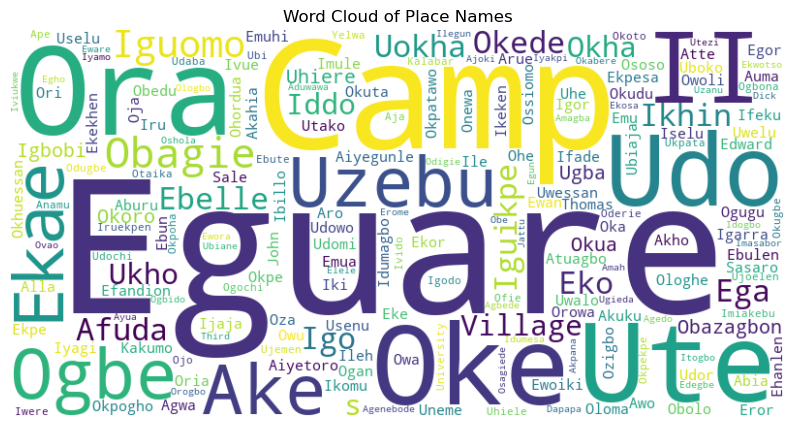
\includegraphics[width=1\linewidth]{wordcloud.png}
    \caption{Word Cloud of Place Names}
    \label{fig:wordcloud}
\end{figure}
\section{Development of Data Acquisition Algorithms and Information Model for Place Names and Attributes}
I developed the Software Requirements Specification (SRS) document to provide the information model for recording data describing place names and their attributes in a systematic manner. Our system stores temporal and spatial location data for places, includes algorithms for gathering data from multiple sources, and provides a tool environment for investigating changes in place names.
The model will serve as a platform for users to discover and learn about various destinations across Edo-Benin City. It will use a large database to produce helpful and engaging content.
\subsubsection{Features}
The Model will connect with a database to store and retrieve information about locations, administrative areas, and other related aspects such as historical data, alternative names, geographical attributes, and user-generated information.

\section*{Key Features}

\begin{itemize}
    \item \textbf{Administrative Details, Locations}: Provide the foundation for understanding the geographical and administrative context of a location.
    \item \textbf{Alternative Names}: Enhance searchability and discovery by incorporating the various names a location may have.
    \item \textbf{Geographical Features}: Offer a deeper understanding of a location's physical characteristics.
    \item \textbf{Historical Data}: Enrich locations with stories and events that occurred throughout time.
\end{itemize}

\subsection*{Functional Requirements}

\begin{itemize}
    \item \textbf{User Management}: 
    \begin{itemize}
        \item Users will be able to register, login, and logout.
        \item The application will authenticate users based on username and password stored securely.
        \item Implement mechanisms to reset forgotten passwords.
        \item An admin user type will exist with elevated privileges.
    \end{itemize}
    \item \textbf{Location Management}:
    \begin{itemize}
        \item Users will be able to search for locations based on various criteria (name, postal code, etc.).
        \item The application will display details of a location, including its description, founding year (if available), and alternative names.
        \item Allow authorized users to add new locations with descriptions and basic details.
    \end{itemize}
    \item \textbf{Content Management}:
    \begin{itemize}
        \item Users will be able to create and submit posts related to locations.
        \item Implement a workflow for approving/rejecting posts by administrators.
        \item Users will be able to view posts associated with specific locations.
        \item Allow users to add comments to existing posts.
    \end{itemize}
    \item \textbf{Administrative Functions}: 
    \begin{itemize}
        \item Admin users can manage user accounts, update administrative details, and potentially manage other aspects of the data.
    \end{itemize}
\end{itemize}

\subsection*{Non-Functional Requirements}

\begin{itemize}
    \item \textbf{Performance}
    \begin{itemize}
        \item The system shall be capable of handling large volumes of data efficiently.
        \item Data retrieval and query processing shall be optimized for responsiveness.
        \item Algorithms for data acquisition shall be designed for scalability and performance.
    \end{itemize}
    \item \textbf{Security}
    \begin{itemize}
        \item Access to the system shall be role-based, with different levels of permissions for users.
        \item Data stored within the system shall be encrypted to ensure confidentiality and integrity.
        \item Measures shall be in place to prevent unauthorized access and data breaches.
    \end{itemize}
    \item \textbf{Reliability}
    \begin{itemize}
        \item The system shall be designed with redundancy and failover mechanisms to ensure high availability.
        \item Data integrity checks shall be performed regularly to detect and prevent corruption.
        \item Backup and recovery procedures shall be implemented to mitigate the risk of data loss.
    \end{itemize}
\end{itemize}
\subsection{Data Model (Database Schematic) Diagram}
Below is the model schematic diagram that provide overall model functionality features, 

\section*{Diagram Descriptions}

\begin{description}

    \item[\texttt{administrativedetails}] This table likely stores administrative area information such as country, state, and local government.

    \item[\texttt{administrative\_ass}] This table might store associations between administrative areas and some identifier (\texttt{location\_id}) during a specific period.

    \item[\texttt{admin\_actions}] This table could track actions taken by administrators on the system, including affected users or posts.

    \item[\texttt{alternativenames}] This table likely stores alternative names for locations.

    \item[\texttt{comments}] This table stores information about comments made on posts, including the content and user who created it.

    \item[\texttt{geographicalfeatures}] This table stores geographical features associated with locations, including type, location data, and descriptions.

    \item[\texttt{historical\_data}] This table stores historical data/events related to locations, including event descriptions, sources, and dates.

    \item[\texttt{locations}] Stores information about specific locations, including name, postal code, founding year, and descriptions.

    \item[\texttt{posts}] This table stores posts created by users, including content, approval status, and creation time.

    \item[\texttt{users}] This table stores information about users, including username, password, email, profile information, and account status.

\end{description}

\newpage

\begin{figure}
    \centering
    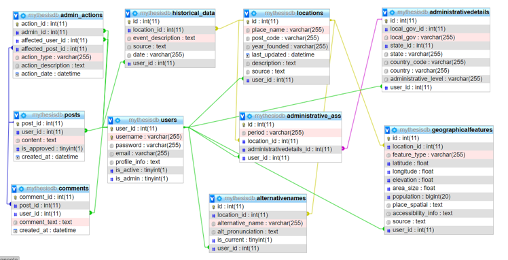
\includegraphics[width=1\linewidth]{model_schema.png}
    \caption{Data Model (Database Schematic) Diagram}
    \label{fig:enter-label}
\end{figure}
\newpage
\section{conclusion}
The study integrates historical, linguistic, archeological, and technological methodologies to better understand the evolution of place names in Edo/Benin City. The study emphasizes the role of colonial and indigenous influences, cultural connections, and socio-cultural processes in constructing the toponymic landscape. The established data gathering approach and providing powerful tools for deeper investigation and comprehension of place names' historical trajectories.
